\documentclass[./AutomatedMK.tex]{subfiles}


\begin{document}

% ============================================================================================================
\section{Our Approach to Classification}\label{sec:Approach_B}
	In the following, we describe the dataset, our data pre-processing, the astronomical knowledge used to perform feature selection, and how it forms the feature matrix.

The dataset used in these experiments comes from SDSS data run 12, 13, and 14, which was collected using the BOSS spectrograph \citep{Smee, boss}. The data runs collected a combined total of 892,614 spectra. Some of the data was rejected because it was not \textit{spectral} class of O, B, A, F, G, K, and M with subclass of 0 - 9 combined with \textit{luminosity class} of I, II, III, IV, V, VII or that the data was missing a large portion of its spectrum, similarly to the work done in \citeauthor{brice}. The data was also pre-processed by SDSS scientists through the methods presented by \citeauthor{Dawson} and \citeauthor{Stoughton}.

The usable dataset contains 453,378 stellar spectra and 46 of the 420 class combinations. It is important to note that this is real collected data and not simulated data. The distribution of the classes from the dataset is imbalanced, as seen in Fig. \ref{fig:dist_B}. The dataset is balanced using an \textit{Undersampling} method (removing samples) \citep{Japkowicz} and a \textit{Hybrid} (Undersampling + Oversampling) method. An \textit{Oversampling} method (duplicating samples) was used to improve accuracy. This technique is supported by the findings presented in \cite{brice}. The Undersampling method results in each class having 55 samples for a total of 2,530 samples. The Oversampling method results in each class having 57,771 samples for a total of 2,657,466 samples. The Hybrid method results in each class having 20,813 samples for a total of 957,398 samples. For Hybrid and Oversampling methods, when a sample is duplicated the duplicate gets a randomly generated new redshift, which makes it a unique sample.

       % Distribution of classes in dataset
        \begin{figure}
            \centering
            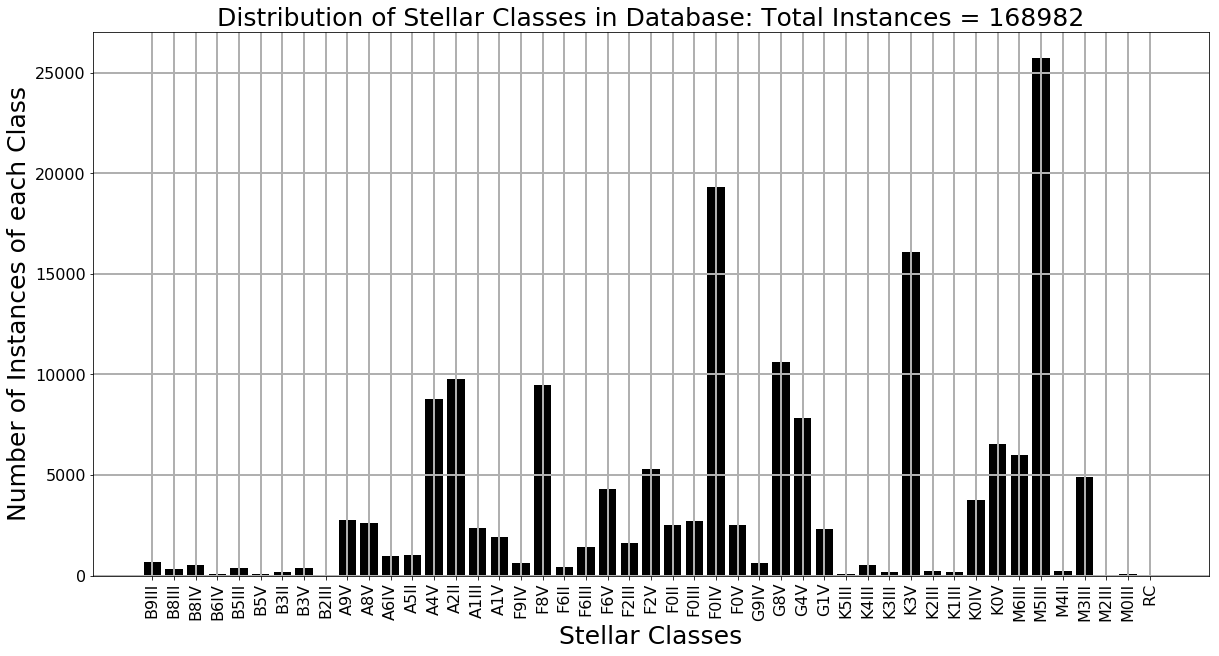
\includegraphics[width=0.5\linewidth]{figures/Distribution_B.png}
            \caption{Distribution of classes in the dataset. RC = Remaining Classes of 0 instances}
            \label{fig:dist_B}
        \end{figure}

The only data pre-processing required for this approach is flux scaling using eq. \eqref{eq:scale}. If a sample is known to have missing or corrupt flux measurements around the absorption lines used for Feature Selection, then an Imputer \footnote{An Imputer is used to fill in missing values in a Feature Matrix. \citet{brice} utilize a moving average Imputer for missing values in stellar spectra.} method is required to fill in missing values. None of the  samples in the dataset used in this analysis required an Imputer.

        % Flux scaling equation
        \begin{equation}\label{eq:scale}
            f_{i, scaled} = \frac{f_i - f_{min}}{f_{max} - f_{min}}
        \end{equation}

where $f_i$ is the \(i\)th  flux measurement, $f_{max}$ and $f_{min}$ are the maximum and minimum flux measurements respectively, and $f_{i, scaled}$ is the resulting scaled flux.

% I could not get the Algorithm section to compile, so I took a picture of it and use this \hyperlink{alg:FS}{1} with this \hypertarget{alg:FS} to mimic the Alorithmic section... 
%Unfortuantly that means that the Algorithm number will not automatically update... But this 
% Paper only has one Algorithm (maybe 2), so it should not be a big deal.

Domain knowledge is used to perform Feature Selection (Algorithm \hyperlink{alg:FS}{1}). It is known that key features of stellar spectra are the absorption lines. Using the standard source "The Classification of Stars" \citep{Jaschek}, an analysis was performed to identify the absorption lines present in each spectral class (O, B, A, F, G, K, and M). 

Redshift makes it impossible to identify the wavelength of any absorption line that is in any given sample. However, the rest wavelength of any absorption line is known. The known rest wavelength of an absorption line can be used to create a set of features (flux measurements) for classification. These set of features are generated by using flux measurements surrounding the rest wavelengths of known absorption lines. It is important note that the absorption line does not have to be present in every sample/class, it is its rest wavelength that is important. The absorption lines used in this study are the H$_\delta$ (4102 $\mathring{A}$) and Ca \RomanNumeralCaps{1} (4227 $\mathring{A}$) lines. Using these two absorption lines, the variability in the intensity and shape of the flux measurements in these regions can separate the samples in the spectral classes and the widths of the line that is present in one or both regions creates separability in the samples for the luminosity classes.

Figures \ref{fig:B}, \ref{fig:A}, \ref{fig:K}, \ref{fig:M}, \ref{fig:F}, \ref{fig:G}, and \ref{fig:2A1} demonstrate how using only the H$_\delta$ and Ca \RomanNumeralCaps{1} lines preserve variability in the intensity, shape, redshift, and widths of the absorption lines needed to classify into the spectral and luminosity classes. The red line is the absorption line at redshift wavelengths, black is at rest wavelengths, and no line means there is no absorption line. Notice in Figs. \ref{fig:B} and \ref{fig:A} (B and A stars) that only the H$_\delta$ absorption line is present, where as Figs. \ref{fig:K} and \ref{fig:M} (K and M stars) only the Ca \RomanNumeralCaps{1} absorption line is present, and Figs. \ref{fig:F} and \ref{fig:G} (F and G stars) both are present. Figure \ref{fig:redP} shows how redshift is preserved because the absorption line is still found within the search space. Figures \ref{fig:B}, \ref{fig:A}, \ref{fig:K}, \ref{fig:M}, \ref{fig:F}, and \ref{fig:G} show that combining these two sets of flux measurements around these absorption lines creates separable samples for the spectral classification. This is achieved because every spectral major class has one or both of these absorption lines. 

Figure \ref{fig:2A1} shows that for two samples with the same spectral class, the width of the absorption line is preserved. As stated in \citep{Gray}, the widths of the absorption lines determine the luminosity classification. 

It is important to note that Algorithm \hyperlink{alg:FS}{1} is embarrassingly parallel and was implemented in parallel for these experiments. Using these two absorption lines results in a feature matrix as seen in Table \ref{tab:feature-matrix2}.

% ----------------------------------------------------- B Star
\begin{sidewaysfigure}[htb!]
\centering

\subfloat[Around the H$_\delta$ absorption line.\label{fig:B4102F}]{%
	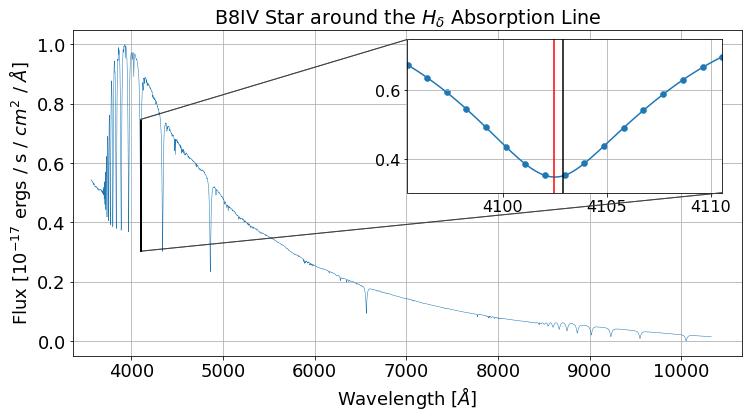
\includegraphics[width=0.4\linewidth]{figures/B4102_Full.png}}
\subfloat[Subplot of (a).\label{fig:B4102}]{%
	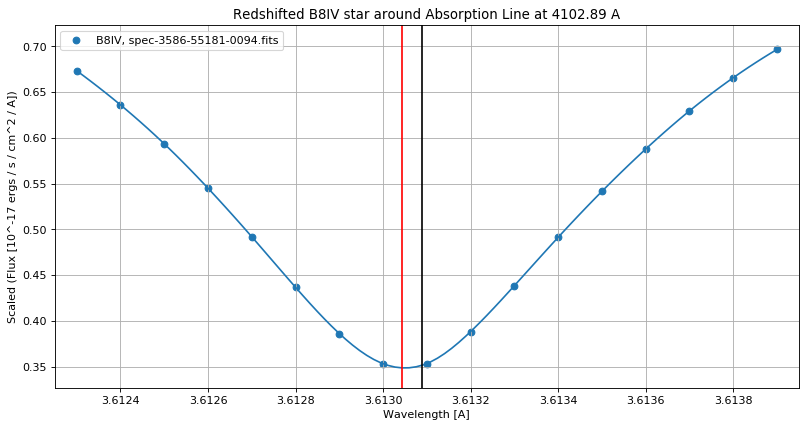
\includegraphics[width=0.4\linewidth]{figures/B4102.png}}

\noindent 

\subfloat[Around the Ca \RomanNumeralCaps{1} absorption line.\label{fig:B4227F}]{%
	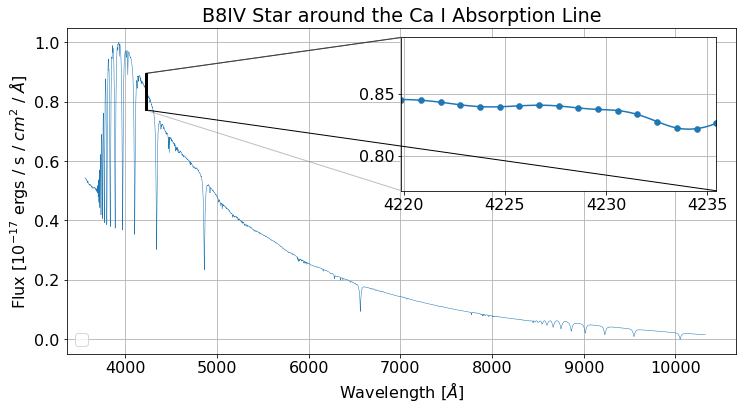
\includegraphics[width=0.4\linewidth]{figures/B4227_Full.png}}
\subfloat[Subplot of (c).\label{fig:B4227}]{%
	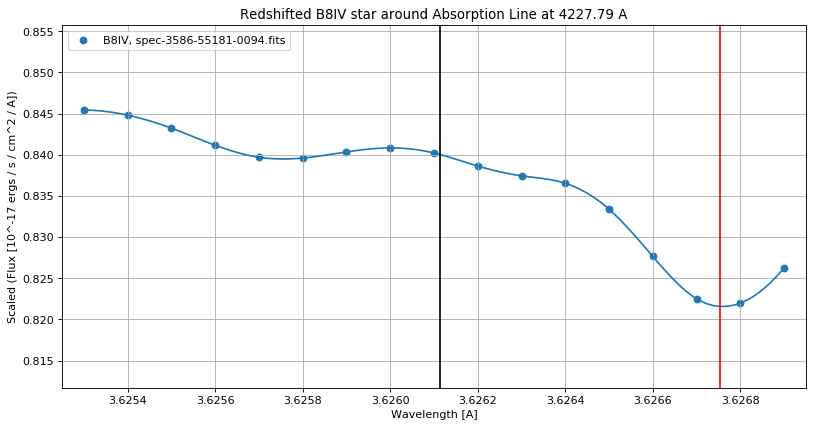
\includegraphics[width=0.4\linewidth]{figures/B4227.png}}

\caption{Example of a B Type Star focusing on wavelengths near $H_\delta$ and Ca \RomanNumeralCaps{1} absorption lines.}
\label{fig:B}
\end{sidewaysfigure}

% ----------------------------------------------------- A Star
\begin{sidewaysfigure}[htb!]
\centering

\subfloat[Around the H$_\delta$ absorption line.\label{fig:A4102F}]{%
	\includegraphics[width=0.4\linewidth]{figures/A4102_Full.png}}
\subfloat[Subplot of (a).\label{fig:A4102}]{%
	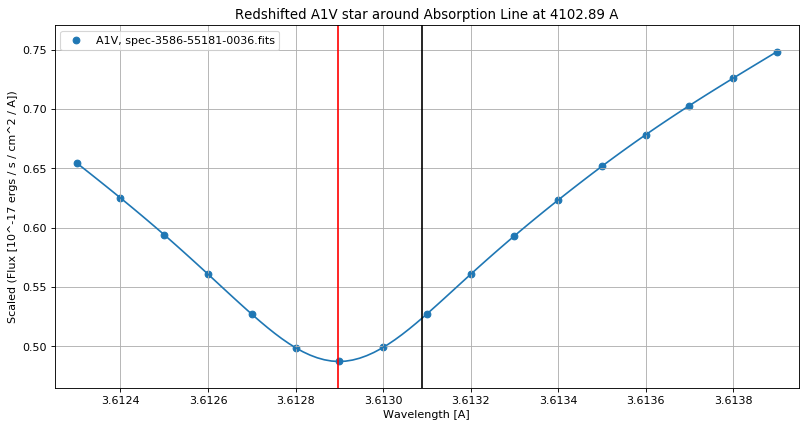
\includegraphics[width=0.4\linewidth]{figures/A4102.png}}

\noindent 

\subfloat[Around the Ca \RomanNumeralCaps{1} absorption line.\label{fig:A4227F}]{%
	\includegraphics[width=0.4\linewidth]{figures/A4227_Full.png}}
\subfloat[Subplot of (c).\label{fig:A4227}]{%
	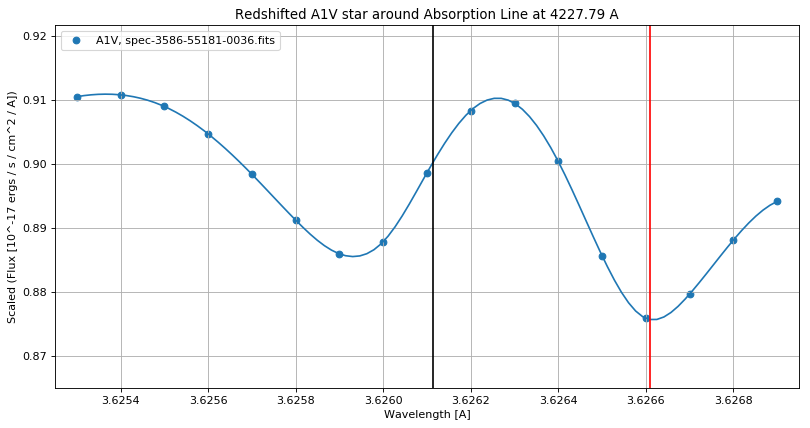
\includegraphics[width=0.4\linewidth]{figures/A4227.png}}

\caption{Example of an A Type Star focusing on wavelengths near $H_\delta$ and Ca \RomanNumeralCaps{1} absorption lines. }
\label{fig:A}
\end{sidewaysfigure}

% ----------------------------------------------------- K Star
\begin{sidewaysfigure}[htb!]
\centering

\subfloat[Around the H$_\delta$ absorption line.\label{fig:K4102F}]{%
	\includegraphics[width=0.4\linewidth]{figures/K4102_Full.png}}
\subfloat[Subplot of (a).\label{fig:K4102}]{%
	\includegraphics[width=0.4\linewidth]{figures/K4102.png}}

\noindent 

\subfloat[Around the Ca \RomanNumeralCaps{1} absorption line.\label{fig:K4227F}]{%
	\includegraphics[width=0.4\linewidth]{figures/K4227_Full.png}}
\subfloat[Subplot of (c).\label{fig:K4227}]{%
	\includegraphics[width=0.4\linewidth]{figures/K4227.png}}

\caption{Example of a K Type Star focusing on wavelengths near $H_\delta$ and Ca \RomanNumeralCaps{1} absorption lines. }
\label{fig:K}
\end{sidewaysfigure}

% ----------------------------------------------------- M Star
\begin{sidewaysfigure}[htb!]
\centering

\subfloat[Around the H$_\delta$ absorption line.\label{fig:M4102F}]{%
	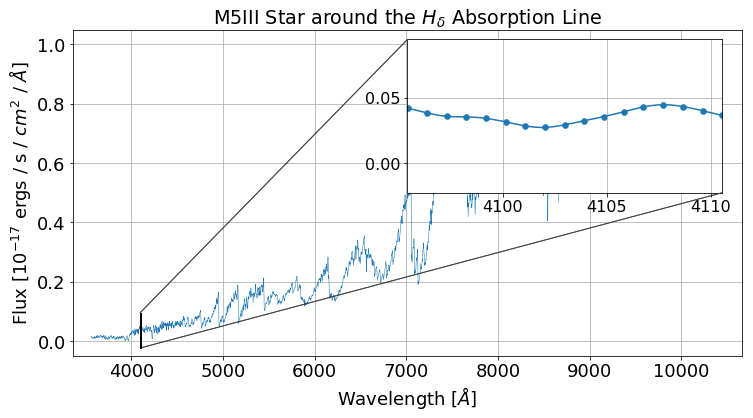
\includegraphics[width=0.4\linewidth]{figures/M4102_Full.png}}
\subfloat[Subplot of (a).\label{fig:M4102}]{%
	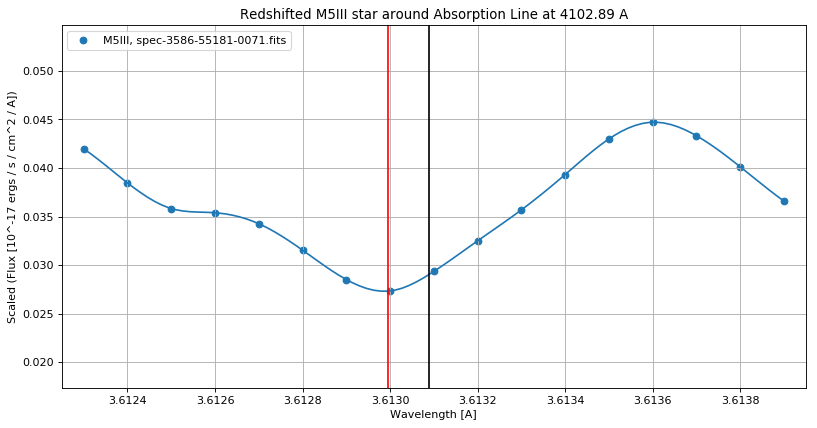
\includegraphics[width=0.4\linewidth]{figures/M4102.png}}

\noindent 

\subfloat[Around the Ca \RomanNumeralCaps{1} absorption line.\label{fig:M4227F}]{%
	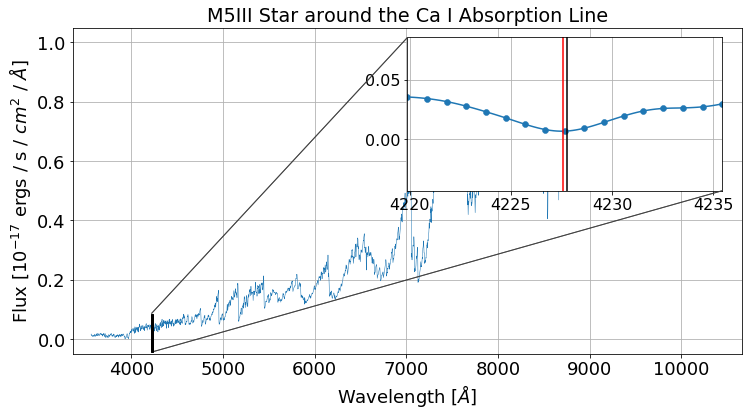
\includegraphics[width=0.4\linewidth]{figures/M4227_Full.png}}
\subfloat[Subplot of (c).\label{fig:M4227}]{%
	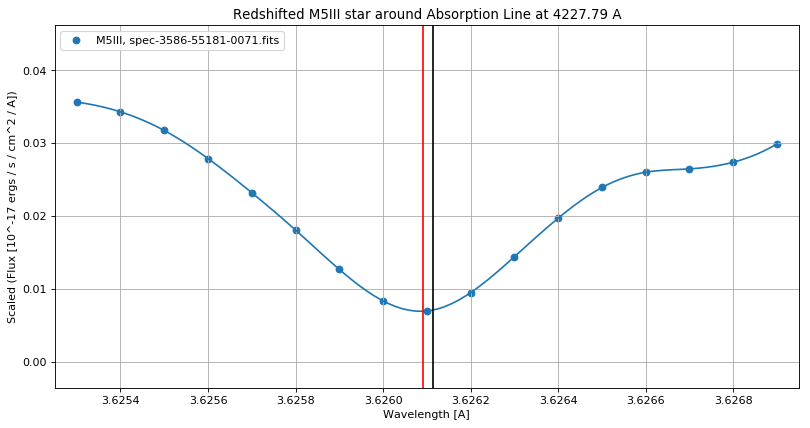
\includegraphics[width=0.4\linewidth]{figures/M4227.png}}

\caption{Example of a M Type Star focusing on wavelengths near $H_\delta$ and Ca \RomanNumeralCaps{1} absorption lines. }
\label{fig:M}
\end{sidewaysfigure}

% ----------------------------------------------------- F Star
\begin{sidewaysfigure}[htb!]
\centering

\subfloat[Around the H$_\delta$ absorption line.\label{fig:F4102F}]{%
	\includegraphics[width=0.4\linewidth]{figures/F4102_Full.png}}
\subfloat[Subplot of (a).\label{fig:F4102}]{%
	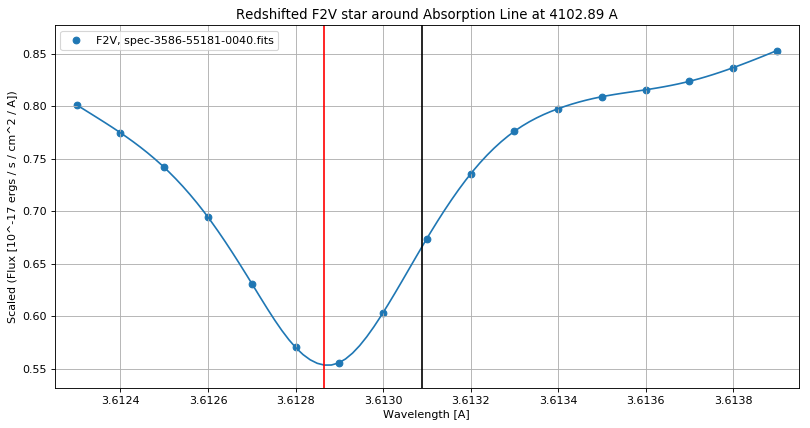
\includegraphics[width=0.4\linewidth]{figures/F4102.png}}

\noindent 

\subfloat[Around the Ca \RomanNumeralCaps{1} absorption line.\label{fig:F4227F}]{%
	\includegraphics[width=0.4\linewidth]{figures/F4227_Full.png}}
\subfloat[Subplot of (c).\label{fig:F4227}]{%
	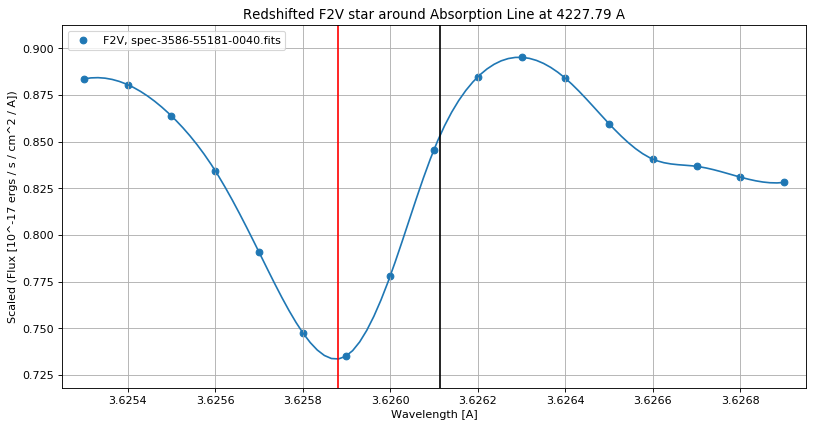
\includegraphics[width=0.4\linewidth]{figures/F4227.png}}

\caption{Example of a F Type Star focusing on wavelengths near $H_\delta$ and Ca \RomanNumeralCaps{1} absorption lines. }
\label{fig:F}
\end{sidewaysfigure}

% ----------------------------------------------------- G Star
\begin{sidewaysfigure}[htb!]
\centering

\subfloat[Around the H$_\delta$ absorption line.\label{fig:G4102F}]{%
	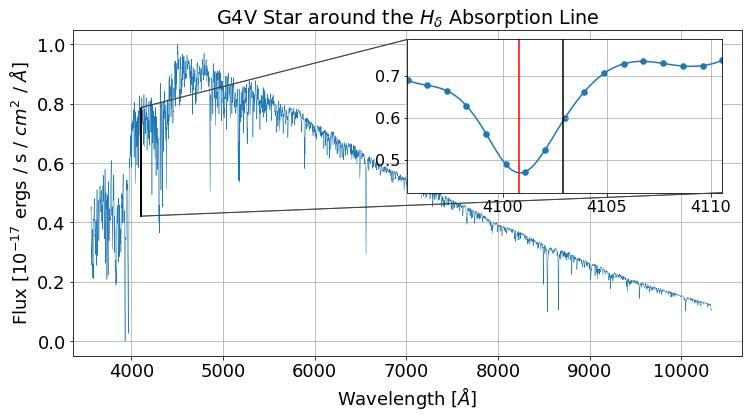
\includegraphics[width=0.4\linewidth]{figures/G4102_Full.png}}
\subfloat[Subplot of (a).\label{fig:G4102}]{%
	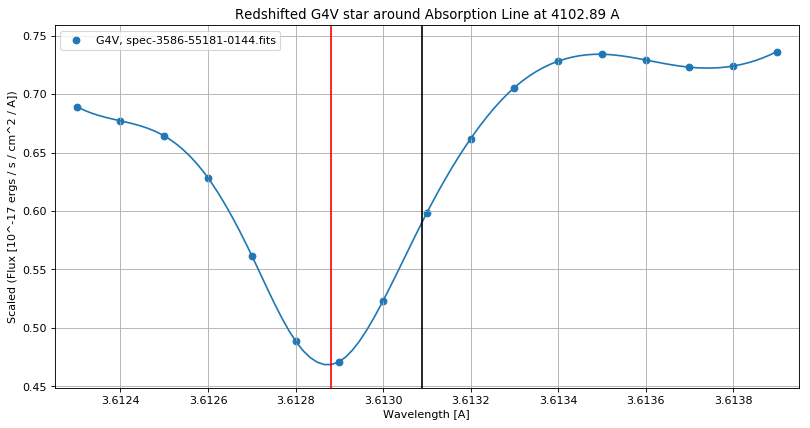
\includegraphics[width=0.4\linewidth]{figures/G4102.png}}

\noindent 

\subfloat[Around the Ca \RomanNumeralCaps{1} absorption line.\label{fig:G4227F}]{%
	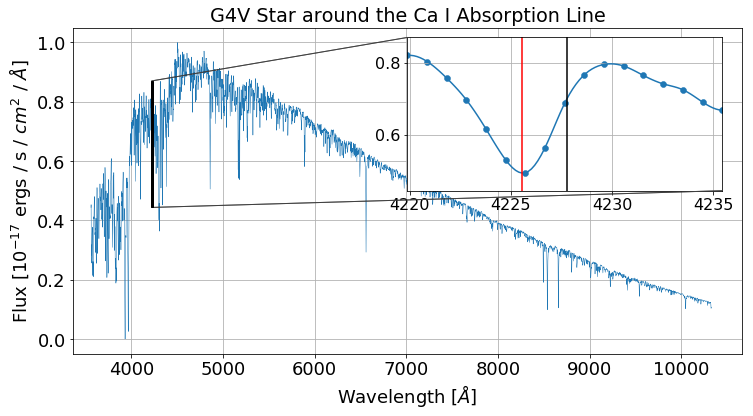
\includegraphics[width=0.4\linewidth]{figures/G4227_Full.png}}
\subfloat[Subplot of (c).\label{fig:G4227}]{%
	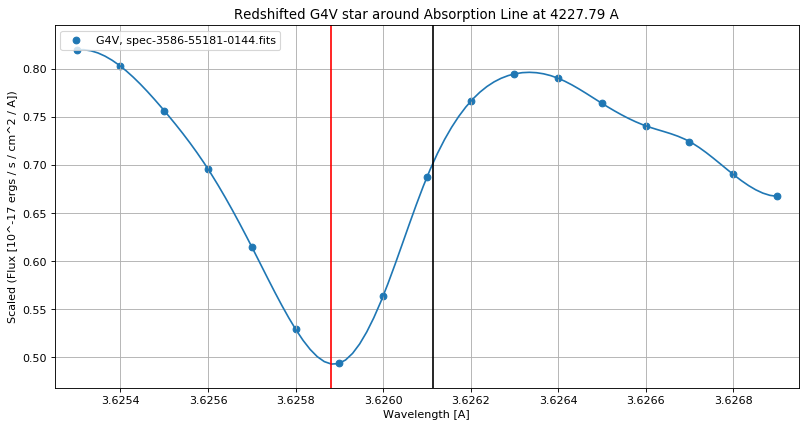
\includegraphics[width=0.4\linewidth]{figures/G4227.png}}

\caption{Example of a G Type Star focusing on wavelengths near $H_\delta$ and Ca \RomanNumeralCaps{1} absorption lines. }
\label{fig:G}
\end{sidewaysfigure}

\begin{figure}[htb!]
\centering
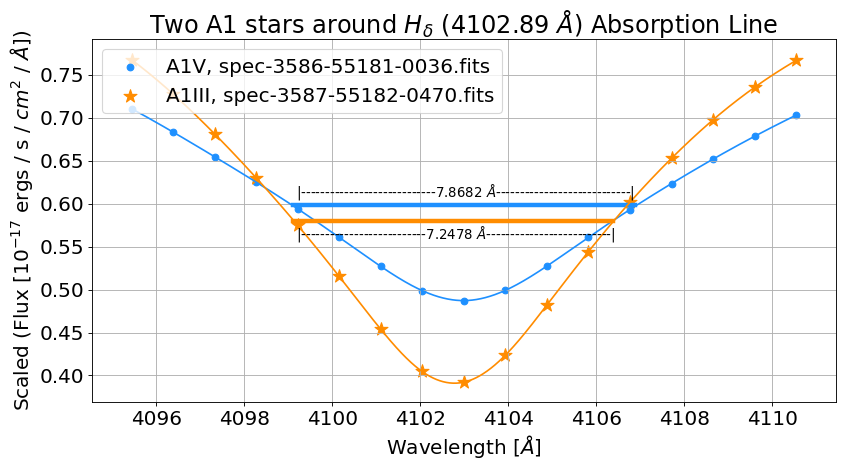
\includegraphics[width=.5\linewidth]{figures/2A1.png}
\caption{Example of the same Harvard class with different wavelength width (Full Width Half Max) for the same absorption line for different MK classes.}
\label{fig:2A1}
\end{figure}

\begin{figure}[htb!]
\centering
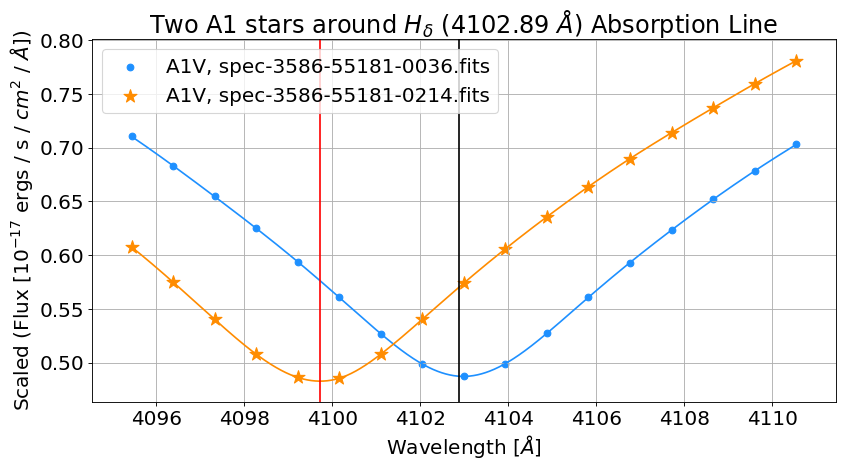
\includegraphics[width=.5\linewidth]{figures/Red_Example.png}
\caption{Example of how Redshift is preserved.}
\label{fig:redP}
\end{figure}

% I could not get the algorithm section / code to generate in aasTex. I took a picture of it and found a hyper link work around so it looks like it works.
% I included the code for the algorithm section in a different email if you would like to attempt getting it to work
% ----------------------------------------------------
\begin{figure}[htb!]
 \hypertarget{alg:FS}
\centering
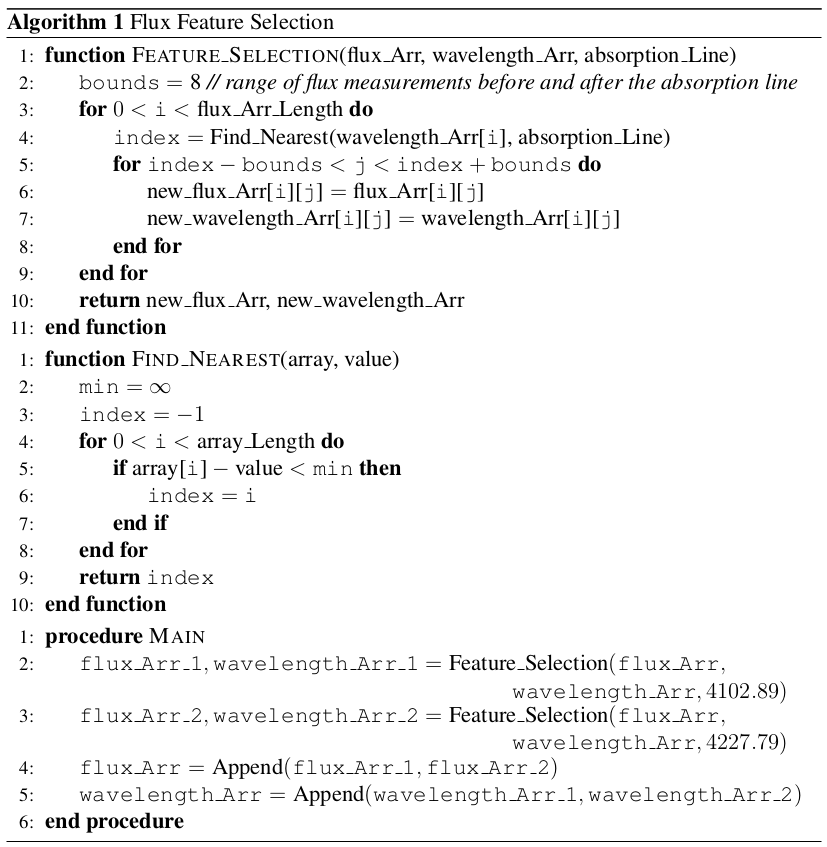
\includegraphics[width=.7\linewidth]{figures/Algorithm1.png}
\label{alg:FS}
\end{figure}

        Each stellar spectra has a wavelength array and an array of corresponding flux measurements. The feature matrix is constructed using 17 flux measurements around the $H_\delta$ (4102 $\mathring{A}$) and 17 flux measurements around the Ca \RomanNumeralCaps{1} (4227 $\mathring{A}$) absorption line (see Table \ref{tab:feature-matrix2}).

A problem arises with the feature matrix because redshift causes the flux measurements to be shifted in wavelength. This is illustrated in Table \ref{tab:example}.     

\begin{table}
\renewcommand{\thetable}{\arabic{table}}
\centering

\caption{Example of the feature matrix using two sets of wavelengths around two absorption lines for a total of 34 features} 
\label{tab:feature-matrix2}

	\begin{tabular}{|c|c|c|c||c|c|c|}
\tablewidth{0pt}
	\hline
			     & Wavelength:   & ... &  Wavelength:	 & Wavelength:   & ... & Wavelength:  \\
  			     & 4,095.43 $\mathring{A}$          &     &  4,110.55 $\mathring{A}$         & 4,219.88 $\mathring{A}$          &     &  4,235.45 $\mathring{A}$ \\ \hline
	Spectrum 1 & Flux                   & ... & Flux                   & Flux                   & ... & Flux                   \\ \hline
	Spectrum 2 & Flux                   & ... & Flux                   & Flux                   & ... & Flux                   \\ \hline
	\end{tabular}

\end{table}

\pagebreak
        % Example of redshift in the feature matrix
        \begin{table}
        \renewcommand{\thetable}{\arabic{table}}
        \centering
        \caption{Example of the feature matrix that has redshifted data}
        \label{tab:example}

            \begin{tabular}{|c|c|c|c|c|c|}
\tablewidth{0pt}
            \hline 
	Star & Wavelength: & Wavelength:	& Wavelength: & Wavelength: & Wavelength: \\
	Class & 6,560.8 $\mathring{A}$ & 6,561.8 $\mathring{A}$ & 6,562.8 $\mathring{A}$ & 6,563.8 $\mathring{A}$ & 6,564.8 $\mathring{A}$  \\ \hline
               A0 & & H$\alpha$ & & &\\ \hline
               A0 & H$\alpha$ & & & & \\ \hline
               A0 & & & H$\alpha$ & & \\ \hline
               A0 & & & & H$\alpha$ & \\ \hline
               A0 &H$\alpha$ & & & &  \\ \hline
            \end{tabular}
        
        \end{table}
\end{document}